\documentclass[a4paper,12pt]{article}

% Margins
\usepackage{geometry}
\geometry{left=25mm,right=25mm,%
bindingoffset=0mm, top=20mm,bottom=20mm}

% More Math Symbols
\usepackage{amssymb}

% Trademark Symbols
\usepackage{textcomp}

% Text in math
\usepackage{amsmath}

% For Diagrams
\usepackage{graphicx}
\usepackage{wrapfig}

% Footnote URLs
\usepackage{hyperref}

% Underlines
\usepackage{soul}

% Font
\usepackage{anyfontsize}
%\usepackage[default,regular,black]{sourceserifpro}
\usepackage{tgpagella,eulervm}
\usepackage[T1]{fontenc}

% Mutli-column text
\usepackage{multicol}

% For tables
\usepackage[table]{xcolor}
\usepackage{array}
\usepackage{tablefootnote}

% Title
\newcommand{\linia}{\rule{\linewidth}{0.5pt}}
\makeatletter
\renewcommand{\maketitle}{
\begin{center}
\vspace{2ex}
{\huge \textbf{\@title}}
\vspace{1ex}
\\
\linia\\
\textsf{\@date \hfill
\@author}
\vspace{4ex}
\end{center}
}
\makeatother
% Multicol TOC
\linespread{1.2}
\makeatletter
\renewcommand\tableofcontents{%
    \section*{\makebox[\linewidth][c]{\contentsname}%
      \@mkboth{\MakeUppercase\contentsname}{\MakeUppercase\contentsname}}%
    \begin{multicols}{2}%
    \@starttoc{toc}%
    \end{multicols}
    }
\makeatother

% Short negative symbol in math mode (sub-zero mnemonic)
\newcommand{\sz}{\text{-}}


% Names
\newcommand{\esp}{\texttt{ESP-32WROOM}}
\newcommand{\con}{\textit{Console}}

% Headers
\usepackage{fancyhdr}
\usepackage{lastpage}
\pagestyle{fancy}
\lhead{}
\chead{}
\rhead{}
\lfoot{Final Project}
\cfoot{}
\rfoot{Page \thepage \ of \pageref{LastPage}}
\renewcommand{\headrulewidth}{0pt}
\renewcommand{\footrulewidth}{0pt}

\begin{document}
% Setting the fontsize
\fontsize{14}{16}\selectfont

\title{Final Project --- AU Robotics}

\date{29/10/2024}

\author{\textbf{Team B}}

\maketitle

\section*{Preface}

This report serves as a technical overview of everything that has been worked on in the past two weeks by Team B in the final project for AU Robotics in 2024.\\

\tableofcontents
\newpage
\part{Software}
\section{Overview \& Dataflow} \label{dataflow}
\subsection{Motion Dataflow} \label{motflow}
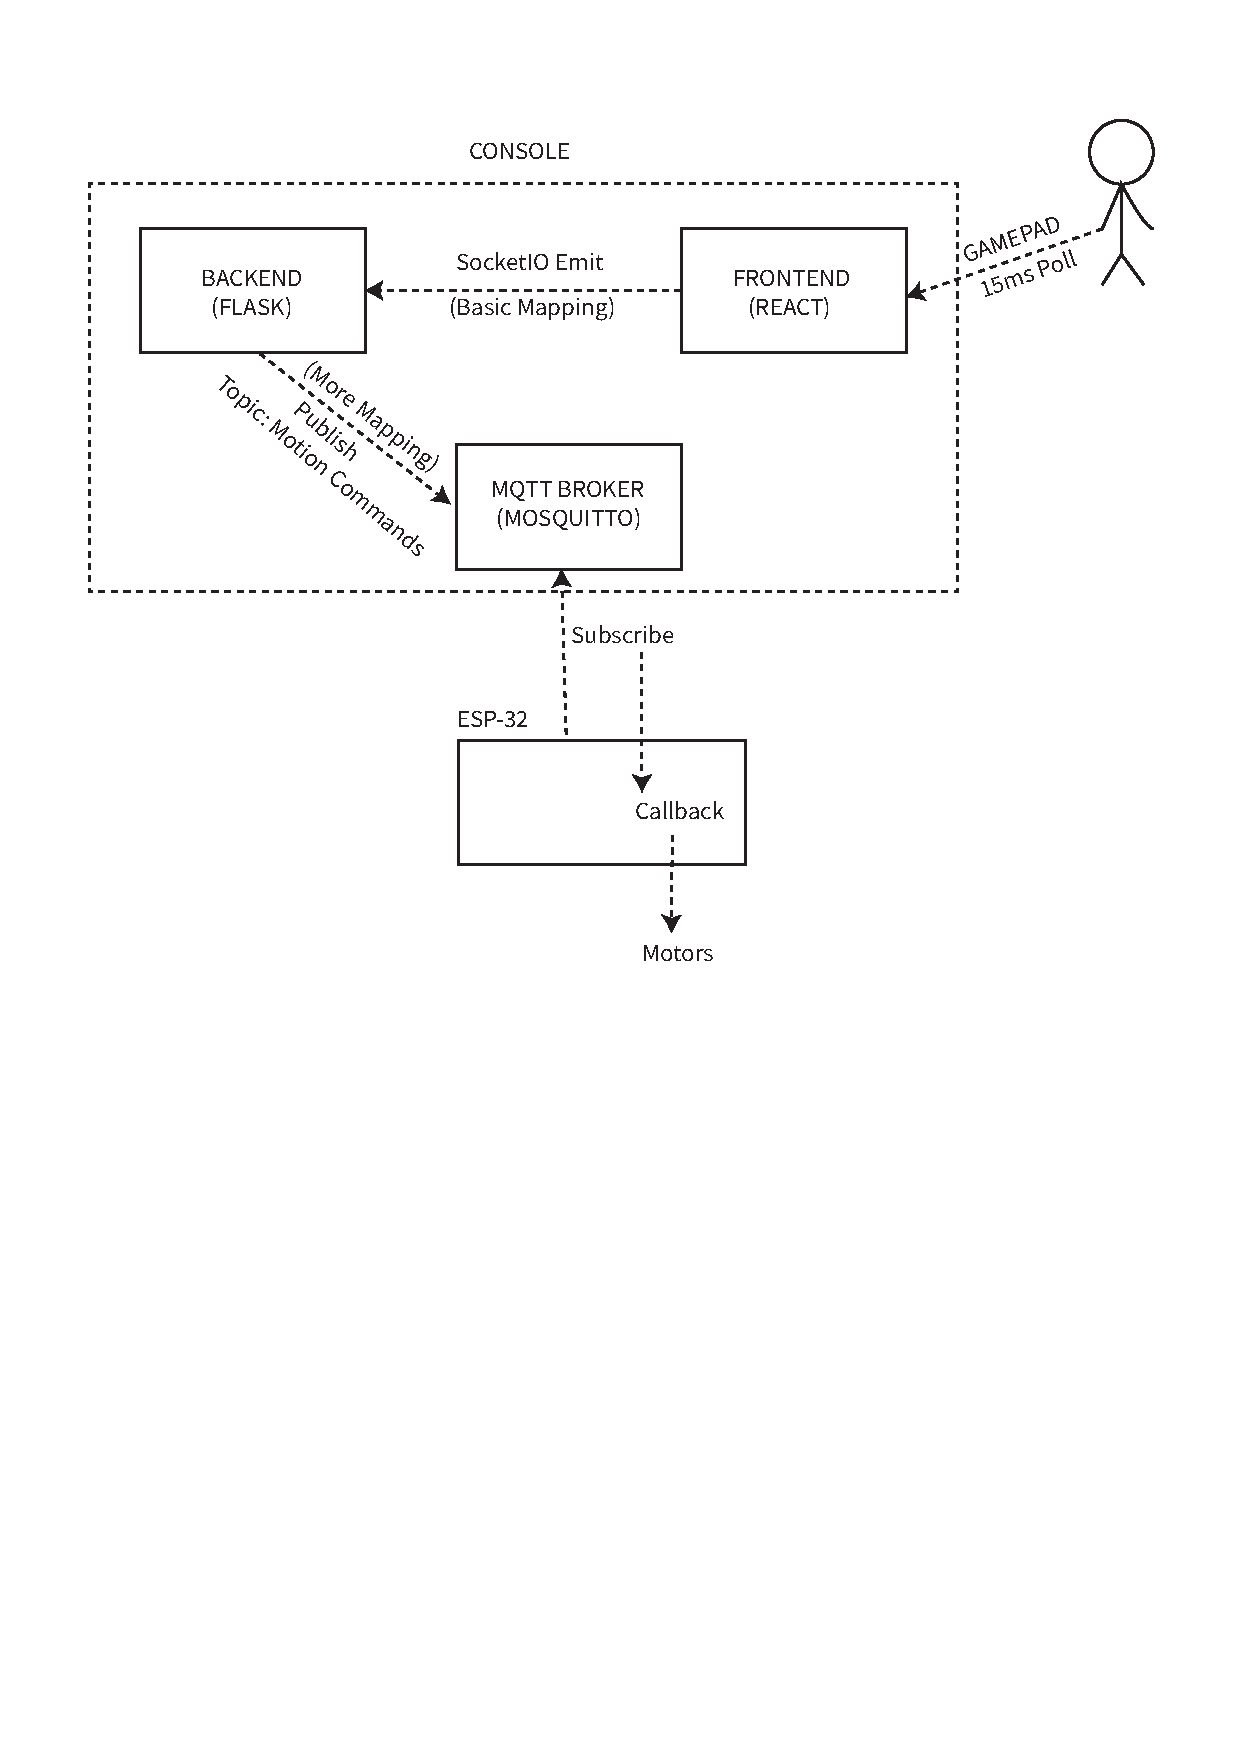
\includegraphics[trim=40 380 0 57,scale=0.95,clip]{diagrams/mot.pdf}

\subsection{Localization Dataflow} \label{locflow}
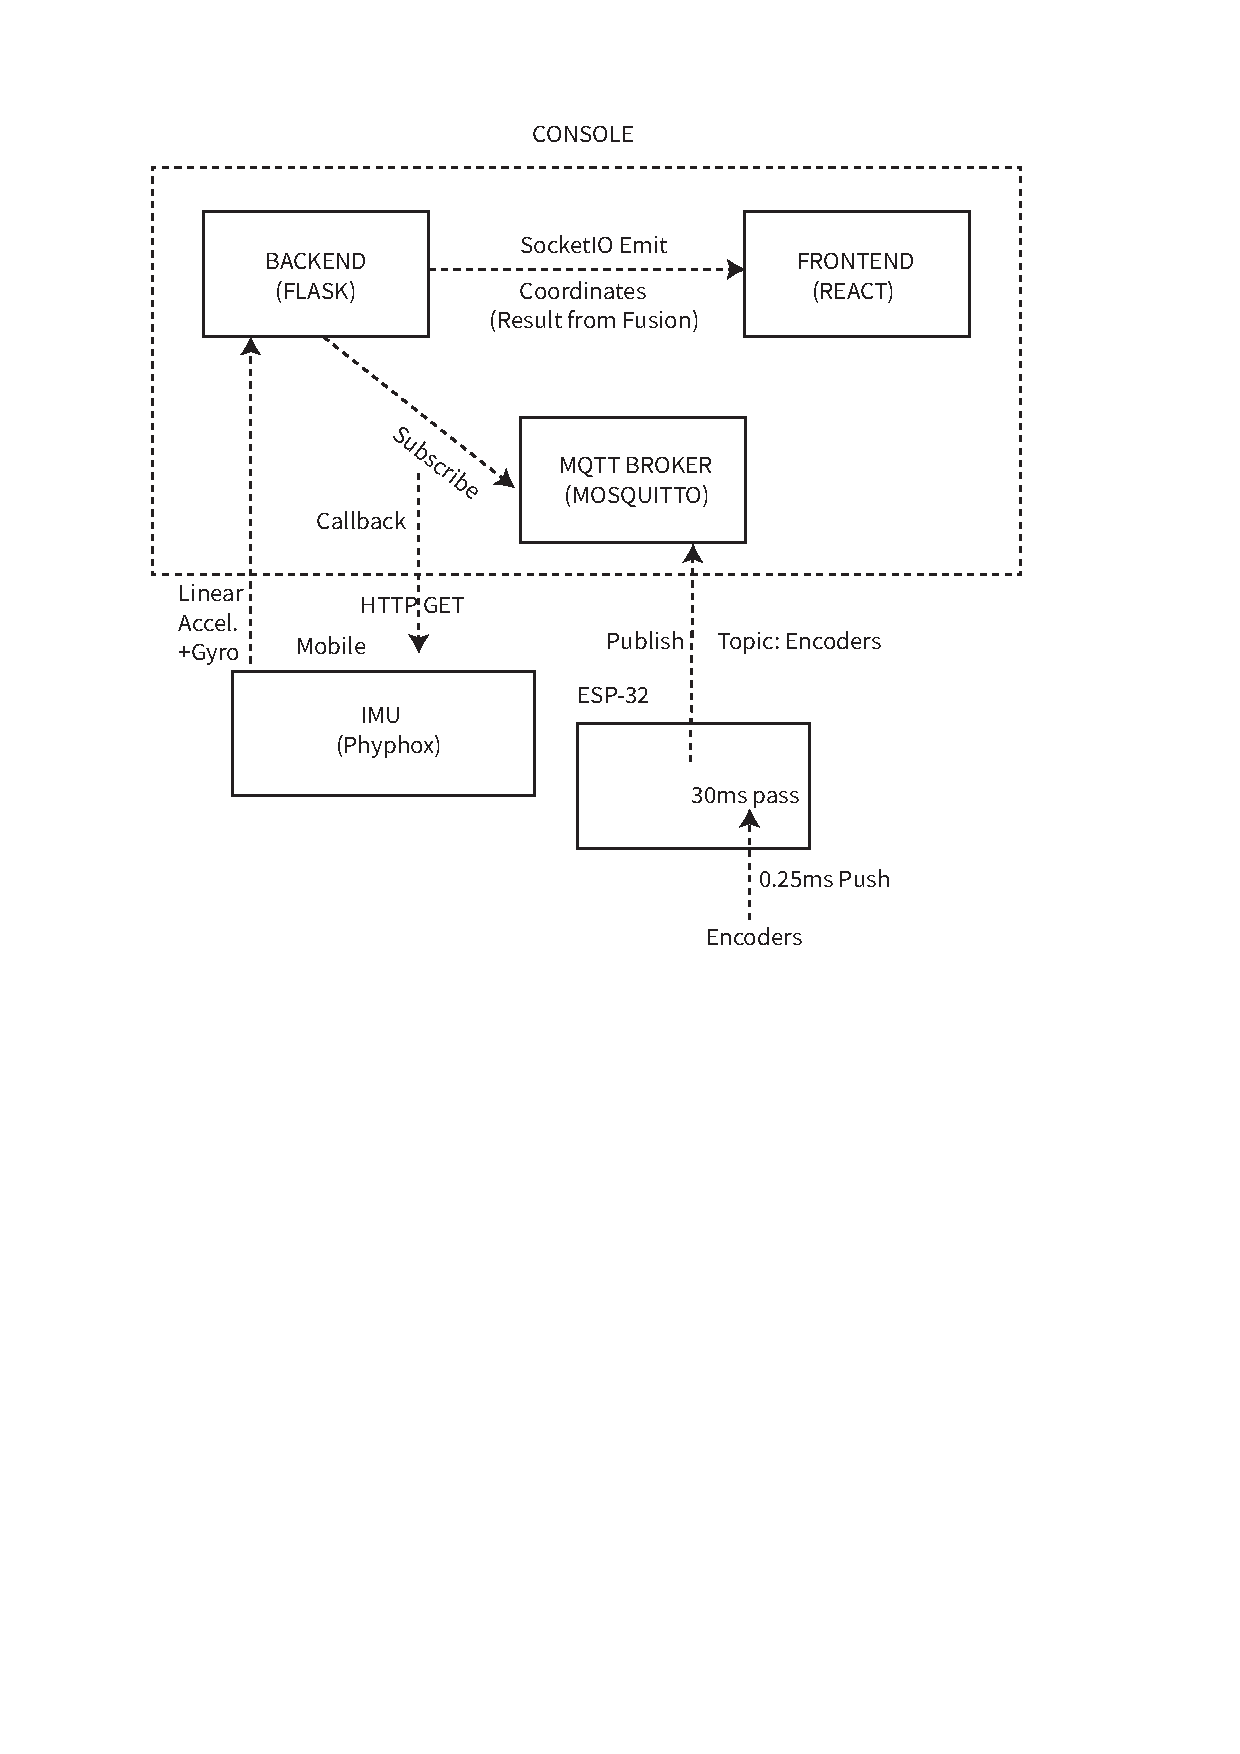
\includegraphics[trim=40 380 0 57,scale=0.95,clip]{diagrams/loc.pdf}

\subsection{Computer Vision Dataflow} \label{visflow}
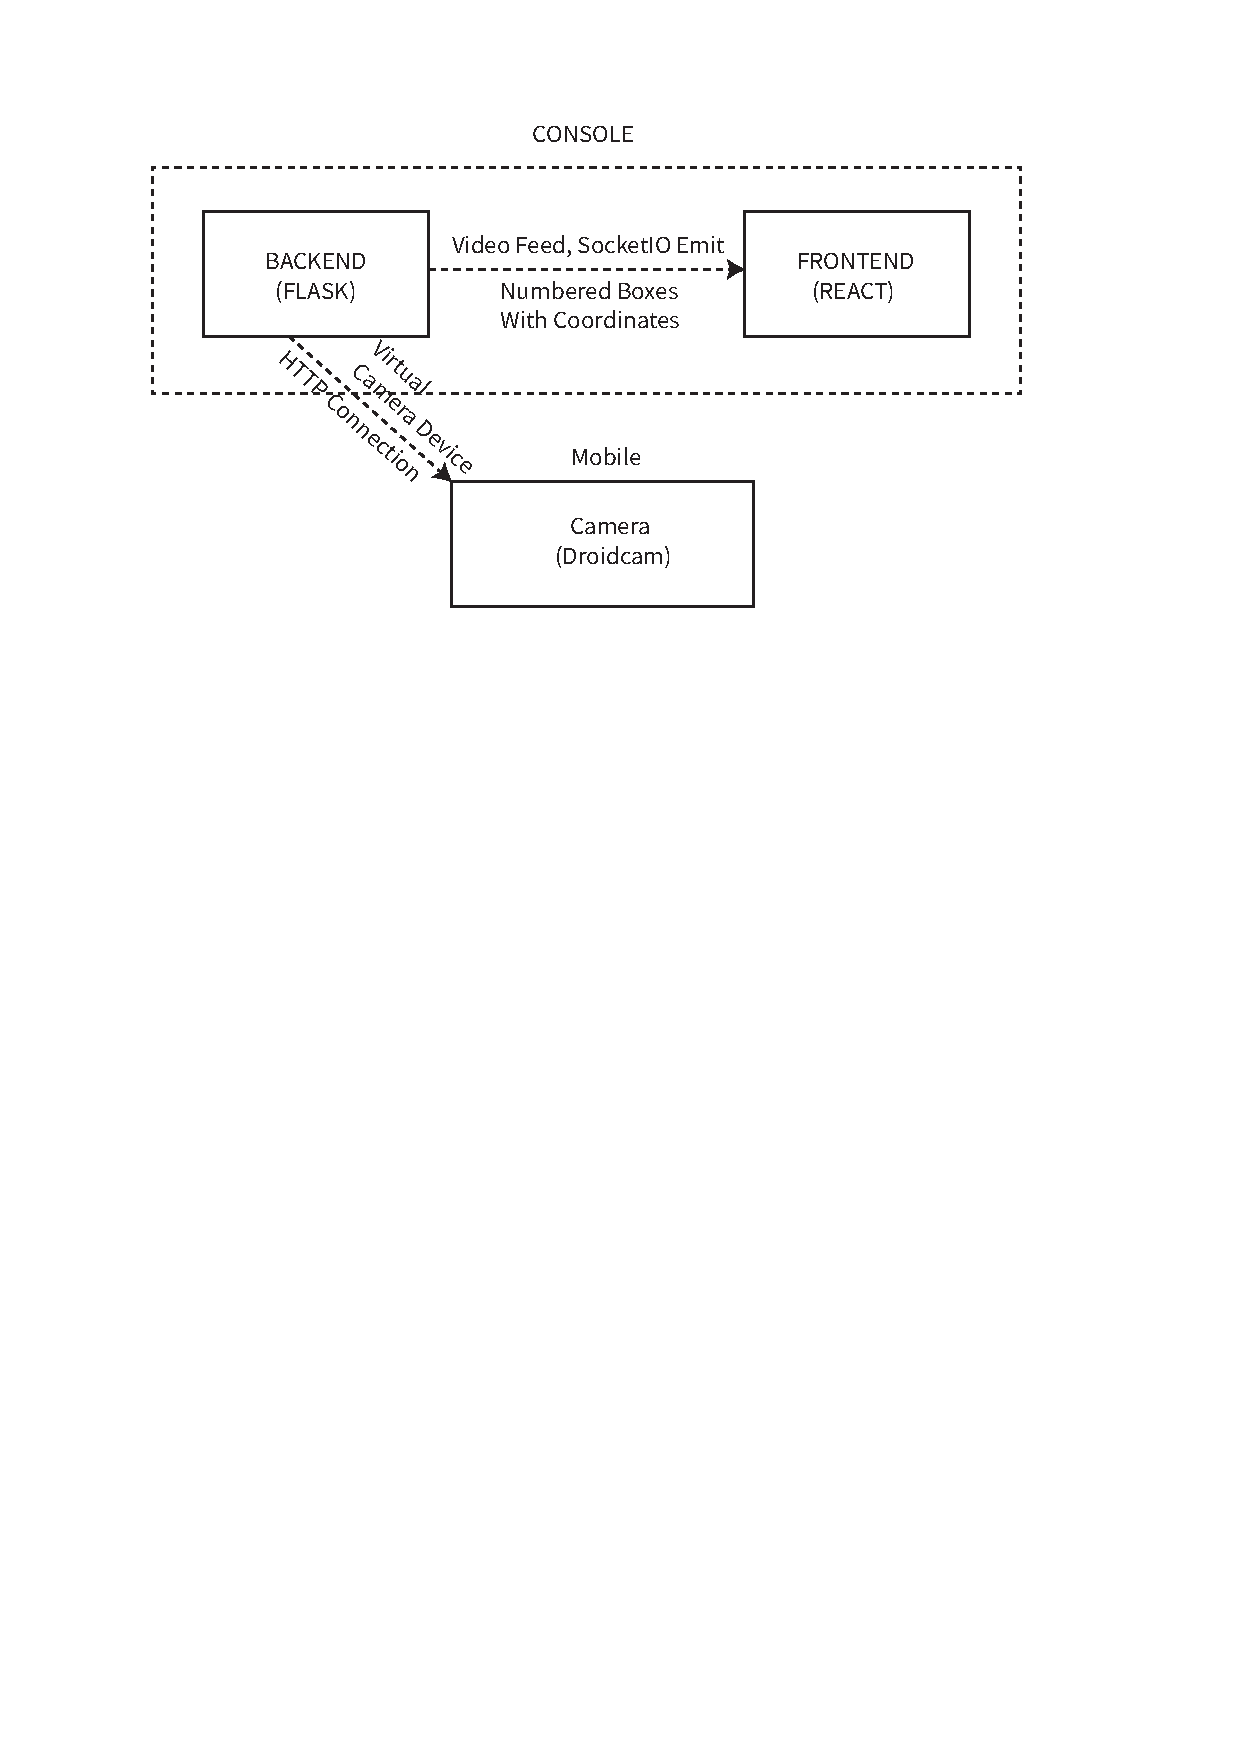
\includegraphics[trim=40 550 0 57,scale=0.95,clip]{diagrams/vis.pdf}

\section{Console}

The \con\ is the powerhouse that all things computable get pushed to. As an extension, it also orchestrates much of the communication between the devices and processes the video feed for detection and decoding of QR codes.

All this is an aside to its main function: allowing the user to control the robot, navigate the map, and track objectives.
The \con\ contains the following UI components:
\begin{itemize}
    \item[(1)] A video feed display, with buttons to set the vision algorithm
    \item[(2)] A dynamic list of all boxes and their respective coordinates
    \item[(3)] A dynamic map being updated with the robot's position
\end{itemize}
\subsection{Navigation \& Control}

Using the Gamepad API\footnote{\url{https://developer.mozilla.org/en-US/docs/Web/API/Gamepad_API}} which is standard in all mainstream web browsers, we are able to process gamepad button presses in a game-loop--like algorithm which polls the gamepad every 15ms.

The algorithm assigns \textit{precedence} to certain inputs, so for example, if the user moves the analog stick used for rotation and also presses the trigger used for forward motion, the algorithm only sends the rotation movement.\\
This is the command format along with the precedence for each command:
\begin{center}
    \bgroup
    \def\arraystretch{1.5}
    {\rowcolors{0}{white!70!gray!70}{white!90!gray!70}
    \begin{tabular}{|l|l|l|p{6em}|}
        \hline
        \textbf{Index} & \textbf{DS$^*$ Button} & \textbf{Command} & \textbf{Value}\\
        \hline
        0 & $\times$ & Arm Down & 0 \\
        \hline
        0 & $\triangle$ & Arm Up & 1 \\
        \hline
        1 & $\bigcirc$ & Grip Close & 0 \\
        \hline
        1 & $\square$ & Grip Open & 1 \\
        \hline
        2 & R2/ L2  & Both Wheels $\uparrow$/ $\downarrow$ & $\sz1 \rightarrow 1$ \\
        \hline
        3 & R Stick $\rightarrow$/ $\leftarrow$ & One Wheel (Rotation) & $\sz1 \rightarrow 0 :$ left \newline $0 \rightarrow 1:$ right\\
        \hline
    \end{tabular}}
    \egroup

    \footnotesize{$^*$ DualShock \textregistered\ or DualSense \textregistered\ which belong to Sony \texttrademark}\\
\end{center}

The reason for using this precedence is to avoid damaging the wheels' differential, by allowing only one type of motion to go through.

As clarification for the forward and backward motion, the command's value is calculated by subtracting the L2 value form the R2 value and sending the command accordingly.

The right analog stick is calibrated using the controller's firmware by doing a full rotation while connected to the \con\ before running the robot, and a further error of $0.1$ in any direction is accounted for --- the vertical directions are disregarded as are all other inputs.

\subsection{Computer Vision}
The role of computer vision is to detect and decode the QR codes on every box and assign a box number to each code, allowing the individual in charge of navigation to effectively track which boxes need to go where.

The algorithms that are made available:
\begin{center}
    \bgroup
    \def\arraystretch{1.5}
    {\rowcolors{0}{white!70!gray!70}{white!90!gray!70}
    \begin{tabular}{|c|c|c|}
        \hline
        \textbf{Library} & \textbf{Strengths} & \textbf{Weaknesses} \\
        \hline
        \texttt{pyzbar} & Extremely Efficient & Angled Codes \\
        \hline
        \texttt{cv2 -- builtin} & Angled Codes & Less Efficient \\
        \hline
        \texttt{qreader} & Deepest Detection & Least Efficient \\
        \hline
    \end{tabular}}
    \egroup
\end{center}
The individual in charge of navigation will be able to switch between the algorithms on-the-fly or even disable them completely. This would also be useful in cases of autonomous or semi-autonomous navigation.
\subsection{Communication}
Several of the communication components are hosted directly, either partly or fully, on the \con.
\begin{center}
    \bgroup
    \def\arraystretch{1.5}
    {\rowcolors{0}{white!70!gray!70}{white!90!gray!70}
    \begin{tabular}{|c|c|c|}
        \hline
        \textbf{Host} & \textbf{Component} & \textbf{Connects to} \\
        \hline
        Mobile & IMU & \con\ w/ HTTP GET \\
        \hline
        Mobile & Camera & \con\ w/ HTTP \\
        \hline
        \con & \texttt{MQTT Broker} & \esp \\
        \hline
        \con\ -- Backend & Flask \& SocketIO & Frontend \\
        \hline
    \end{tabular}}
    \egroup
\end{center}

Mutlithreading for the different event handlers is handled graciously by the libraries used (\texttt{Flask}, \texttt{Flask-SocketIO}, \texttt{Paho-MQTT}). As an example, \texttt{Paho-MQTT}'s \texttt{loop\_start} and \texttt{loop\_stop} are used instead of the thread-blocking \texttt{loop\_forever} which requires manual thread handling.

The full dataflow is illustrated in Section \ref{dataflow}.

\section{Embedded}
\subsection*{Goals}
Programming the \esp\ to do the following:
\begin{itemize}
    \item receive motion commands from the console and translate them into something the motors can understand
    \item translate commands related to the arm and gripper into something the servo can understand
    \item send encoder data to the console to enable it to carry out its localization routine
\end{itemize}
\section{Localization \& Motion}
\subsection*{Goals}

With the power of the laptop used for the \con, the localization team should efficiently and accurately calculate the coordinates.

The team will receive the encoder readings from the \esp\ as shown in Section \ref{locflow}.There is little communication overhead with the \esp\ due to the fact that the \texttt{MQTT Broker} is running locally on the \con.
After receiving the encoder data, the IMU readings --- which are the linear acceleration in the $x$ direction, and the angular acceleration in the $z$ direction --- are requested from the mobile phone mounted on the robot.

A Kalman filter will be performed on the accelerations to obtain their respective velocities, then fusion of all the data will be performed to calculate the current coordinates and dispatch them to the frontend.

\section{Setup Instructions}
Setup instructions for every software component will be indicated and updated in the repository's various README files.
The repository will be hosted remotely at 
\end{document}